\chapter{Equations and inequalities}
\setcounter{figure}{1}
\setcounter{subfigure}{1}

\section{Solving linear equations}
\nopagebreak
 $ \hspace{-5pt}\begin{array}{cccccccccccc}   
\includegraphics[width=0.75cm]{col11306.imgs/summary_fullmarks.png} &   
\includegraphics[width=0.75cm]{col11306.imgs/summary_video.png} &   \end{array} $ \hspace{2 pt}\raisebox{-5 pt}{} {(section shortcode: MG10068 )} \par 
           
The simplest equation to solve is a linear equation. A linear equation is an
equation where the highest exponent of the variable is $1$. The
following are examples of linear equations:\par 


\begin{equation*}
\begin{array}{ccl}\hfill 2x+2& =& 1\hfill \vspace{6pt} \\
 \hfill \dfrac{2-x}{3x+1}& =& 2\hfill \vspace{6pt} \\
\hfill 4(2x-9)-4x&=&4-6x \hfill  \vspace{6pt}\\ 
\hfill \dfrac{2a-3}{3}-3a&=&\dfrac{a}{3} \hfill\\
\end{array}
\end{equation*}
Solving an equation means finding find the value of the variable that makes
the equation true. For example, to solve this simple equation $x+1=1$, we need to determine the value of $x$ that will make the left hand side equal to the right hand side. The solution is $x=0$.\par 
The solution, also called the root of an equation, is the value of the variable that satisifes the equation.
For linear equations, there is at most one solution for the equation.\par 
To solve equations we use algebraic methods that include expanding expressions, grouping terms and factorising.\par 

\begin{equation*}
  \begin{array}{ccll}\hfill 2x+2& =& 1\hfill \\ 
      \hfill 2x& =& 1-2\hfill & \mbox{(rearrange)}\hfill \\ 
      \hfill 2x& =& -1\hfill & \mbox{(simplify)}\hfill \\
\hfill x&=& -\frac{1}{2} & \mbox{(divide both sides by $2$)} \hfill
  \end{array}
\end{equation*}

\begin{equation*}

\end{equation*}
Check the answer by substituting $x=-\frac{1}{2}$ back into the original equation:

\begin{equation*}
    \begin{array}{ccl}\hfill \mbox{LHS}& =& 2x+2\hfill \\
	  & =& 2(-\frac{1}{2})+2\hfill \\
	  & =& -1+2\hfill \\
	  & =& 1\hfill \\
	  \hfill \mbox{RHS}& =& 1\hfill \\
    \end{array}
\end{equation*}
Therefore $x = -\frac{1}{2}$ is a valid solution.

\Tip{When you have found the solution to an equation,
check your answer by substituting the solution back into the original equation.}

\subsection*{Method for solving linear equations}

The general steps for solving linear equations are:
\begin{enumerate}[noitemsep, label=\textbf{\arabic*}. ] 
    \item  Expand all brackets.
    \item Rearrange the equations so that all terms containing the variable are one on side of the equation and all constant terms are on the other side.
    \item  Group like terms together and simplify.
\item Factorise if necessary.
    \item  Find the solution and write down the answer.
    \item Check the answer by substituting the solution back into the original equation.
\end{enumerate}

\Tip{An equation must always be balanced; whatever you do to the left hand side, you must also do to the right hand side.}

\setcounter{subfigure}{0}
\begin{figure}[H] % horizontal\label{m39241*equations-1}
\textnormal{Khan academy video on equations - 1}\vspace{.1in} \nopagebreak
\label{m39241*yt-media1}\label{m39241*yt-video1}
\raisebox{-5 pt}{ 
\includegraphics[width=0.5cm]{col11306.imgs/summary_www.png}} { (Video:  MG10069 )}
\vspace{2pt}   $\theta $
    &

\vspace{.1in}
\end{figure}       

    
\begin{wex}{Solving linear equations }
{
Solve for $x$: $15-2x=3$
}
{
\westep{Rearrange the terms}

\begin{equation*}
    \begin{array}{cclc}\hfill 15-2x& =& 3\hfill & \\
	    \hfill -2x& =& 3-15\hfill & \hfill 
	    
    \end{array}
\end{equation*}

\westep{Simplify}
\begin{equation*}
    \begin{array}{cccc}\hfill -2x& =&-12\hfill & 
	    
    \end{array}
\end{equation*}

\westep{Divide both sides by $-2$}
\begin{equation*}
    \begin{array}{cccc}\hfill x& =&6\hfill & 
	    
    \end{array}
\end{equation*}
\westep{Check answer by substituting solution back into original equation}  

\begin{equation*}
\begin{array}{ccc}\hfill 15 - 2(6)& =& 3\hfill \\
 \hfill 15-12& =& 3\hfill \\
\hfill 3 &=& 3\hfill
\end{array}
\end{equation*}
Since both sides are equal, the answer is correct. 
}
\end{wex}

\begin{wex}
{Solving linear equations }
{Solve for $x$: $4(2x-9)-4x=4-6x$}
{
\westep{Expand the brackets and simplify}

\begin{equation*}
    \begin{array}{ccl}\hfill 4(2x-9)-4x& =& 4-6x\hfill  \\ 
	\hfill 8x-36-4x& =& 4-6x\hfill   \\ 
	\hfill 8x-4x+6x& =& 4+36\hfill  \\ 
	\hfill (8x-4x+6x)& =& (4+36)\hfill   \\   
	\hfill 10x& =& 40\hfill  
    \end{array}
\end{equation*}

\westep{Divide both sides by $10$}
\begin{equation*}
    \begin{array}{ccl}
	\hfill \dfrac{10}{10}x& =& \dfrac{40}{10}\hfill\\
	\hfill x& =& 4\hfill  
    \end{array}
\end{equation*}

\westep{Check answer by substituting solution back into original equation}  

\begin{equation*}
    \begin{array}{ccl}\hfill 4[2(4)-9]-4(4)& =& 4-6(4)\hfill \\
	\hfill 4(8-9)-16& =& 4-24\hfill \\
	\hfill 4(-1)-16& =& -20\hfill \\
	\hfill -4-16& =& -20\hfill \\
	\hfill -20& =& -20\hfill 
    \end{array}
\end{equation*}
Since both sides are equal, the answer is correct. 
}
\end{wex}

\begin{wex}{Solving linear equations }
{Solve for $x$: $\dfrac{2-x}{3x+1}=2$} 
{
\westep{Multiply both sides of the equation by $(3x+1)$}
Division by $0$ is not permitted so there must be a restriction ($x\neq -\frac{1}{3}$)

\begin{equation*}
    \begin{array}{ccll}\hfill \dfrac{2-x}{3x+1}& =& 2\hfill & \\
	\hfill (2-x)& =& 2(3x+1)\hfill & \\ 
    \end{array}
\end{equation*}

\westep{Expand brackets and simplify}
\begin{equation*}
    \begin{array}{ccll}
	\hfill 2-x& =& 6x+2\hfill & \hfill \\ 
	\hfill -x-6x& =& 2-2\hfill & \hfill \\ 
	\hfill -7x& =& 0\hfill & \hfill
    \end{array}
\end{equation*}

\westep{Divide both sides by $-7$}
\begin{equation*}
    \begin{array}{ccll}

	\hfill x& =& \dfrac{0}{-7}\hfill & \\
	\hfill x& =& 0\hfill & \hfill 
    \end{array}
\end{equation*}
Note that $0$ divided by any number is equal to $0$.

\westep{Check answer by substituting solution back into original equation}

\begin{equation*}
    \begin{array}{ccc}\hfill \dfrac{2-(0)}{3(0)+1}& =& 2\hfill \vspace{6pt}\\
	\hfill 2& =& 2\hfill 
\end{array}
\end{equation*}
Since both sides are equal, the answer is correct.
}
\end{wex}


\begin{wex}
{Solving linear equations}
{Solve for $a$: $\dfrac{2a-3}{3}-3a=\dfrac{a}{3}$}
{
\westep{Multiply the equation by common denominator $3$ and simplify}  

\begin{equation*}
    \begin{array}{cccc}\hfill 2a-3 - 9a &= &a\hfill & \\ 
\hfill -7a - 3 &= &a\hfill & 
    \end{array}
\end{equation*}

\westep{Rearrange terms and simplify}
\begin{equation*}
    \begin{array}{cccc}\hfill -7a -a &= &3\hfill & \\ 
\hfill -8a &= &3\hfill & \\
    \end{array}
\end{equation*}

\westep{Divide both sides by $-8$} 
\begin{equation*}
    \begin{array}{cccc}\hfill a &= & -\dfrac{3}{8}\hfill & \\ 

    \end{array}
\end{equation*}

\westep{Check answer by substituting solution back into original equation}
\begin{equation*}
    \begin{array}{ccll}\hfill \dfrac{2(-\frac{3}{8}) - 3}{3} - 3(-\frac{3}{8}) &= & \dfrac{-\frac{3}{8}}{3}\hfill & \\ 
\\
      \hfill \dfrac{(-\frac{3}{4}) - \frac{12}{4}}{3} + \frac{9}{8} &= & \dfrac{-\frac{3}{8}}{3}\hfill & \\ 
\\
 \hfill \Bigg[-\frac{15}{4} \times \frac{1}{3}\Bigg] + \frac{9}{8} &= & -\frac{3}{8} \times \frac{1}{3}\hfill & \\ 
\\
 \hfill -\frac{5}{4} + \frac{9}{8} &= & -\frac{1}{8}\hfill & \\ 
 \hfill -\frac{10}{8} + \frac{9}{8} &= & -\frac{1}{8}\hfill & \\ 
 \hfill -\frac{1}{8} &= & -\frac{1}{8}\hfill & 
    \end{array}
\end{equation*}
Since both sides are equal, the answer is correct. 
}
\end{wex}

\begin{exercises}{}
{
Solve the following equations: \\
Assume all denominators are non-zero.
\begin{multicols}{2}
\begin{enumerate}[noitemsep, label=\textbf{\arabic*}. ] 
\item   $2y-3=7$
\item   $-3y=0$        
\item   $16y+4=-10$        
\item   $12y+0=144$
\item   $7+5y=62$   \vspace{6pt}     
\item  $55=5x+\dfrac{3}{4}$ \vspace{6pt}
\item   $5x=2x+45$        
\item  $23x-12=6+3x$
\item   $12-6x+34x=2x-24-64$
\item   $6x+3x=4-5(2x-3)$
\item   $18-2p=p+9$   \vspace{6pt}
\item   $\dfrac{4}{p}=\dfrac{16}{24}$
\item   $-(-16-p)=13p-1$
\item   $3f-10=10$
\item   $3f+16=4f-10$
\item   $10f+5=-2f-3f+80$
\item   $8(f-4)=5(f-4)$
\item  $6=6(f+7)+5f$      
\item $(a-1)^{2} - 2a = (a+3)(a-2) - 3$
\item $-7x = x+8(1-x)$ \vspace{6pt}
\item $5-\dfrac{7}{b} = \dfrac{2(b+4)}{b}$\vspace{6pt}
\item $\dfrac{x+2}{4} - \dfrac{x-6}{3} = \dfrac{1}{2}$\vspace{6pt}
\item $ 3 - \dfrac{y-2}{4} = 4$\vspace{6pt}
\item $ \dfrac{a+1}{a+2} = \dfrac{a-3}{a+1}$
  
\end{enumerate}
\end{multicols}
\par \raisebox{-5 pt}{
\includegraphics[width=0.5cm]{col11306.imgs/summary_www.png}} Find the answers with the shortcodes:
\par \begin{tabular}[h]{cccccc}
(1.) lcR  &  (2.) lcR  &  (3.) lcR  &  (4.) lcR  &  (5.) lcR  &  (6.) lcn  &  (7.) lcn  &  (8.) lcn  &  (9.) lcn  &  (10.) lcn  &  (11.) lcQ  &  (12.) lcQ  &  (13.) lcQ  &  (14.) lcQ  &  (15.) lcQ  &  (16.) lcU  &  (17.) lcU  &  (18.) lcU  &  (19.) lcU  &  (20.) lcU  & \end{tabular}
}
\end{exercises}

\section{Solving quadratic equations}

 $ \hspace{-5pt}\begin{array}{cccccccccccc}   
\includegraphics[width=0.75cm]{col11306.imgs/summary_fullmarks.png} &   
\includegraphics[width=0.75cm]{col11306.imgs/summary_video.png} &   \end{array} $ \hspace{2 pt}\raisebox{-5 pt}{} {(section shortcode: MG10070 )}       \par
A quadratic equation is an equation where the exponent of the variable is at most
$2$. \\The following are examples of quadratic equations:\par 


\begin{equation*}
    \begin{array}{ccl}\hfill 2{x}^{2}+2x& =& 1\hfill \\
	\hfill 3{x}^{2}+2x-1&=&0 \\ 
	\hfill 0&=&-2{x}^{2}+4x-2\hfill 
    \end{array}
\end{equation*}

Quadratic equations differ from linear equations in that a linear
equation only has one solution, while a quadratic equation has at most
two solutions. There are some special situations, however, in which a quadratic equation only
has one solution.

\begin{activity}{}
Solve the quadratic equation $x^{2}=16$ using the following three different methods:
\begin{enumerate}[noitemsep, label=\textbf{\arabic*}. ] 
\item Inspection (trial and error)
\item Taking the square root
\item Factorising
\end{enumerate}
(Note that if $a \times b = 0$ then $a = 0$ or $b=0$)
\end{activity}

We solve quadratic equations using factorisation. For example in order to solve $2{x}^{2}-x-3 = 0$

we need to write it in its equivalent factorised form, as $(x+1)(2x-3)=0$.


\subsection*{Method for solving quadratic equations}
\begin{enumerate}[noitemsep, label=\textbf{\arabic*}. ] 
\item Rewrite the equation in the required form $ax^{2} +bx +c =0$.
\item Divide the entire equation by any common factor of the coefficients,
to obtain an equation of the form $a{x}^{2}+bx+c=0$ where $a$, $b$ and
$c$ have no common factors.
\\For example, $2{x}^{2}+4x+2=0$ can be written as
${x}^{2}+2x+1=0$ by dividing by $2$.
\item Factorise $a{x}^{2}+bx+c=0$ to be of the form $(rx+s)(ux+v)=0$.

\item The two solutions are $(rx+s)=0$ or $(ux+v)=0$, so $x = -\dfrac{s}{r}$ or $x=-\dfrac{v}{u}$ respectively.
\item Check your answer by substituting back into the original equation.
\end{enumerate}

% \label{m39247*eip-388}
\setcounter{subfigure}{0}
\begin{figure}[H] % horizontal\label{m39247*equations-3}
\textnormal{Khan academy video on equations - 3}\vspace{.1in} \nSolve 
\label{m39247*yt-media3}\label{m39247*yt-video3}
\raisebox{-5 pt}{ 
\includegraphics[width=0.5cm]{col11306.imgs/summary_www.png}} { (Video:  MG10071 )}
\vspace{2pt}
\vspace{.1in}
\end{figure}

        
\begin{wex}
{Solving quadratic equations }
{Solve for $x$: $3{x}^{2}+2x-1=0$}
{
\westep{The equation is in the required form $ax{2} + bx + c = 0$}

\westep{Factorise}
\begin{equation*}
(x+1)(3x-1)=0
\end{equation*}

\westep{Solve for both solutions}
We have
\begin{equation*}
     \begin{array}{ccc}\hfill x+1&=&0\hfill \\
	\hfill \therefore x&=&-1
    \end{array}
\end{equation*}

or
\begin{equation*}
     \begin{array}{ccc}\hfill 3x-1&=&0\hfill \\
	\hfill \therefore x&=&\frac{1}{3}
    \end{array}
\end{equation*}
\westep{Check both answers by substituting back into the original equation}
\westep{Write final answer}
The solution to $3{x}^{2}+2x-1=0$ is $x=-1$ or $x=\frac{1}{3}$.
}
\end{wex}


\begin{wex}{ Solving quadratic equations }
{Find the roots of the quadratic equation  $0=-2{x}^{2}+4x-2$}
{
\westep{Divide the equation by common factor $-2$}

\begin{equation*}
\begin{array}{ccc}\hfill -2{x}^{2}+4x-2& =& 0\hfill \\ \hfill {x}^{2}-2x+1& =& 0\hfill \end{array}
\end{equation*}

\westep{The equation is in the required form $ax{2} + bx + c = 0$}

\westep{Factorise}
\begin{equation*}
\begin{array}{ccc} \hfill (x-1)(x-1) &=& 0 \hfill \\
\hfill (x-1)^{2} &=&0 \hfill 
\end{array}
\end{equation*}

\westep{The quadratic is a perfect square}
This is an example of a special situation in which there is only one solution to the quadratic equation
\begin{equation*}
\begin{array}{ccc} \hfill x -1 &=& 0 \hfill \\
\hfill \therefore x &=&1 \hfill 
\end{array}
\end{equation*}

\westep{Check your answer by substituting back into the original equation}

 
\westep{Write the final answer}
The solution to $0=-2{x}^{2}+4x-2$ is $x=1$.
}
\end{wex}


\begin{exercises}{ }
{
Solve the following equations:
\begin{multicols}{2}
\begin{enumerate}[noitemsep, label=\textbf{\arabic*}. ] 
\item  $(3x+2)(3x-4)=0$
\item  $(5x-9)(x+6)=0$
\item  $(2y+3)(2y-3)=0$ 
\item  $(2x+1)(2x-9)=0$    
\item  $(4x)(x-3)=-9$       
\item  $20m+25{m}^{2}=0$
\item  $2{x}^{2}-5x-12=0$  
\item  $-75{x}^{2}+290x=240$
\item  $2x=\frac{1}{3}{x}^{2}-3x+14\frac{2}{3}$
\item  ${x}^{2}-4x=-4$      
\item  $-{x}^{2}+4x-6=4{x}^{2}-5x+3$       
\item  ${t}^{2}=3t$  
\item  ${x}^{2}-10x=-25$      
\item  ${x}^{2}=18$
\item  ${p}^{2}-6p=7$
\item  $4{x}^{2}-17x-77=0$
\item  $14{x}^{2}+5x=6$
\item  $2{x}^{2}-2x=12$              
\end{enumerate}
\end{multicols}
\par \raisebox{-5 pt}{
\includegraphics[width=0.5cm]{col11306.imgs/summary_www.png}} Find the answers with the shortcodes:
\par\begin{tabular}[h]{cccccc}
(1.) lcP  &  (2.) lcP  &  (3.) lcP  &  (4.) lcP  &  (5.) lcP  &  (6.) lcE  &  (7.) lcE  &  (8.) lcE  &  (9.) lcE  &  (10.) lcE  &  (11.) lcE  &  (12.) lcm  &  (13.) lcm  &  (14.) lcm  &  (15.) lcm  &  (16.) lcm  &  (17.) lcm  &  (18.) lcm  &  (19.) lcm  & \end{tabular}
}
\end{exercises}
% %          \section{ Exponential equations}
% %     \nopagebreak
% %             \label{m39253} $ \hspace{-5pt}\begin{array}{cccccccccccc}   
\includegraphics[width=0.75cm]{col11306.imgs/summary_fullmarks.png} &   \end{array} $ \hspace{2 pt}\raisebox{-5 pt}{} {(section shortcode: MG10072 )} \par 
% %     
% %     
\section{Solving simultaneous equations}
$ \hspace{-5pt}\begin{array}{cccccccccccc}   
\includegraphics[width=0.75cm]{col11306.imgs/summary_fullmarks.png} &   
\includegraphics[width=0.75cm]{col11306.imgs/summary_video.png} &   \end{array} $ \hspace{2 pt}\raisebox{-5 pt}{} {(section shortcode: MG10076 )} \par

Up to now we have solved equations with only one unknown variable. 
When solving for two unknown variables, two equations are required and these equations are known as simultaneous equations. 
The solutions are the values of the unknown variables which satisfy both equations simultaneously. In general, if there are $n$ unknown variables, then $n$ independent equations are required to obtain a value for each of the $n$ variables.\par 
An example of a system of simultaneous equations:

\begin{equation*}
\begin{array}{rcl} x+y&=&-1 \\ 
 3&=&y-2x 
\end{array}
\end{equation*}

We have two independent equations to solve for two unknown variables. We can solve simultaneous equations algebraically using substitution and elimination methods. We will also show that a system of simultaneous equations can be solved graphically.\par 
\setcounter{subfigure}{0}
\begin{figure}[H] % horizontal\label{m39257*simultaneous-equations}
\textnormal{Khan academy video on simultaneous equations - 1}\vspace{.1in} \nopagebreak
\label{m39257*yt-media7}\label{m39257*yt-video7}
\raisebox{-5 pt}{ 
\includegraphics[width=0.5cm]{col11306.imgs/summary_www.png}} { (Video:  MG10077 )}
\vspace{2pt}
\vspace{.1in}
\end{figure}       

\subsection*{Solving by substitution}
\begin{itemize}
 \item Use the simplest of the two given equations to express one of the variables in terms of the other.
\item Substitute into the second equation. By doing this we reduce the number of equations and the number of variables by one.
\item We now have one equation with one unknown variable which can be solve.
\item Use the solution to substitute back into the first equation to find the value of the other unknown variable.
\end{itemize}

\Note{If the question does not explicitly ask for a graphical solution, then the system of equations should be solved algebraically.}

\begin{wex}
{Simultaneous equations }
{
Solve the following system of equations:
\begin{equation*}
\begin{array}{ccl}\hfill x-y& =& 1\hfill \\ \hfill 3& =& y-2x\hfill \end{array}
\end{equation*}
}
{
\westep{Use the first equation to express $x$ in terms of $y$}
\begin{equation*}
    \begin{array}{ccl}\hfill x& =& y+1\hfill 
    \end{array}
\end{equation*}

\westep{Substitute into the second equation and solve for $y$}
\begin{equation*}
    \begin{array}{ccl}\hfill 3& =& y-2(y+1)\hfill \\
	\hfill 3& =& y - 2y - 2\hfill \\
	\hfill 5& =& -y\hfill \\
\hfill \therefore y& =& -5\hfill
    \end{array}
\end{equation*}

\westep{Substitute back into the first equation and solve for $x$}
\begin{equation*}
    \begin{array}{ccl}\hfill x - (-5)& =& 1\hfill \\
	\hfill x+ 5& =& 1\hfill \\
\hfill \therefore x& =& -4\hfill
    \end{array}
\end{equation*}

\westep{Check the solution by substituting back into both original equations}  

\westep{Write the final answer}
\begin{equation*}
\begin{array}{ccl}\hfill y& =& -5\hfill \\
 \hfill x& =& -4\hfill 
\end{array}
\end{equation*}
}
\end{wex}

\begin{wex}
{Simultaneous equations}
{
Solve the following system of equations:
\begin{equation*}
\begin{array}{ccc}\hfill 4y+3x& =& 100\hfill \\ 
\hfill 4y - 19x& =& 12\hfill 
\end{array}
\end{equation*}
}
{
\westep{Use either equation to express $x$ in terms of $y$}
\begin{equation*}
    \begin{array}{ccl}\hfill 4y+3x & =& 100\hfill \\
\hfill 3x &=& 100 - 4y \hfill \\
\hfill x& =& \dfrac{100 - 4y}{3} \hfill
    \end{array}
\end{equation*}


\westep{Substitute into the second equation and solve for $y$}
\begin{equation*}
    \begin{array}{ccl}\hfill 4y - 19(\dfrac{100 - 4y}{3})& =& 12\hfill \\
	\hfill 12y - 19(100 - 4y)  & =& 36\hfill \\
	\hfill 12y - 1900 + 76y & =& 36 \hfill \\
\hfill  88y& =& 1936 \hfill \\
\hfill \therefore y& =& 22 \hfill
    \end{array}
\end{equation*}

\westep{Substitute back into the first equation and solve for $x$}
\begin{equation*}
    \begin{array}{ccl}\hfill x &=& \dfrac{100 - 4(22)}{3}\hfill \vspace{6pt}\\
	\hfill & =& \dfrac{100-88}{3}\hfill \vspace{6pt}\\
	\hfill & =& \dfrac{12}{3}\hfill\vspace{6pt} \\
	\hfill \therefore x&=& 4 \hfill 
    \end{array}
\end{equation*}

\westep{Check the solution by substituting back into both original equations}  

\westep{Write the final answer}
\begin{equation*}
\begin{array}{ccc}
 \hfill x& =& 4\hfill \\
\hfill y& =& 22\hfill 
\end{array}
\end{equation*}
}
\end{wex}

\subsection*{Solving by elimination}

\begin{wex}
{Simultaneous equations }
{
Solve the following system of equations:
\begin{equation*}
\begin{array}{ccll}\hfill & 3x+y& =& 2\hfill \\ 

\hfill& 6x-y& =& 25\hfill 
\end{array}
\end{equation*}
}
{
\westep{Make the coefficients of either variable in both equations the same}
The coefficients of $y$ in the given equations are $1$ and $-1$. Eliminate the variable $y$ by adding the two equations together
\begin{equation*}
\begin{array}{ccll}\hfill & 3x+y& =& 2\hfill \\ 
\hfill+ & 6x-y& =& 25\hfill \\ \hline
 \hfill & 9x + 0 &=& 27
\end{array}
\end{equation*}


\westep{Simplify and solve for $x$}
\begin{equation*}
    \begin{array}{ccl}\hfill 9x& =& 27\hfill \\
	\hfill \therefore x  & =& 3\hfill 
    \end{array}
\end{equation*}

\westep{Substitute the value of $x$ back into either original equation and solve for $y$}
\begin{equation*}
    \begin{array}{ccl}\hfill 3(3) + y &=& 2\\
	\hfill y & =& 2-9\\
	\hfill \therefore y & =& -7 
   \end{array}
\end{equation*}

\westep{Check the solution $x=3$ and $y=-7$ satisfies both original equations}  

\westep{Write the final answer}
\begin{equation*}
\begin{array}{ccc}
 \hfill x& =& 3\hfill \\
\hfill y& =& -7\hfill 
\end{array}
\end{equation*}
}
\end{wex}

\begin{wex}
{Simultaneous equations }
{
Solve the following system of equations:
\begin{equation*}
\begin{array}{cccc}\hfill & 2a - 3b& =& 5\hfill \\ 
\hfill& 3a-2b& =& 20\hfill 
\end{array}
\end{equation*}
}
{
\westep{Make the coefficients of either variable in both equations the same}
By multiplying the first equation by $3$ and the second equation by $2$, both coefficients of $a$ will be $6$.
\begin{equation*}
\begin{array}{cccc}\hfill & 6a-9b& =& 15\hfill \\ 
\hfill- & (6a-4b& =& 40)\hfill \\ \hline
 \hfill & 0 - 5b &=& -25 

\end{array}
\end{equation*}
(When subtracting two equations, be careful of the signs.)

\westep{Simplify and solve for $x$}
\begin{equation*}
    \begin{array}{ccl}
 \hfill b &=& \dfrac{-25}{-5} \\
 \hfill \therefore b &=& 5
    \end{array}
\end{equation*}

\westep{Substitute the value of $b$ back into either original equation and solve for $a$}
\begin{equation*}
    \begin{array}{ccl}\hfill 2a - 3(5)&=& 5\\
	\hfill 2a-15 & =& 5\\
	\hfill 2a & =& 20\\
	\hfill \therefore a & =& 10 
   \end{array}
\end{equation*}

\westep{Check the solution $a=10$ and $b=5$ satisfies both original equations}  

\westep{Write the final answer}
\begin{equation*}
\begin{array}{ccc}
 \hfill a& =& 10\hfill \\
\hfill b& =& 5\hfill 
\end{array}
\end{equation*}
}
\end{wex}


\subsection*{Solving graphically}

Simultaneous equations can also be solved graphically. If the graphs of each linear equation are drawn, then the solution to the system of simultaneous equations is the co-ordinate of the point at which the two graphs intersect.\par 
For example:
\begin{equation*}
\begin{array}{cc}\hfill x=2y\\ \hfill y=2x-3\end{array}
\end{equation*}

The graphs of the two equations are shown below.\par 

\setcounter{subfigure}{0}
\begin{figure}[H] % horizontal\label{m39257*uid96}
\begin{center}
\rule[.1in]{\figurerulewidth}{.005in} \\
\label{m39257*uid96!!!underscore!!!media}\label{m39257*uid96!!!underscore!!!printimage}
%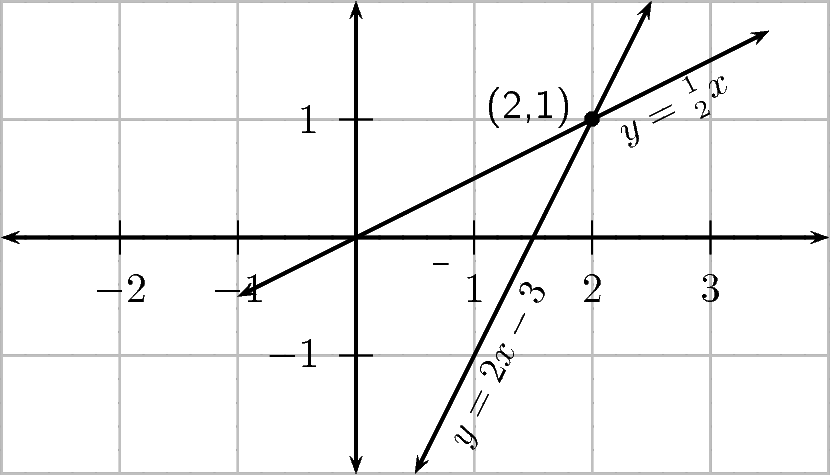
\includegraphics[width=.8\columnwidth]{col11306.imgs/m39257_MG10C10_006.png} % m39257;MG10C10\_006.png;;;6.0;8.5;
\begin{pspicture}(-3,-2)(4,2)
% \psgrid[gridcolor=lightgray,gridlabels=0,gridwidth=0.5pt]
\psaxes[dx=1,Dx=1,arrows=<->](0,0)(-3,-2)(4,2)
\pstextpath[c](-1.1,-0.3){\psplot[xunit=1,plotstyle=curve,arrows=<->]{0.5}{2.5}{x 2 mul 3 sub}}{\small{$y=2x-3$}}
\pstextpath[c](1.5,-0.3){\psplot[xunit=1,plotstyle=curve,arrows=<->]{-1}{3.5}{0.5 x mul}}{\small{$y=\frac{1}{2}x$}}
\uput[l](2,1.1){$(2,1)$}
\psdot(2,1)
\end{pspicture}

\vspace{2pt}
\vspace{.1in}
\rule[.1in]{\figurerulewidth}{.005in} \\
\end{center}
\end{figure}       
The intersection of the two graphs is $(2;1)$. So the solution to the system of simultaneous equations is $x=2$ and $y=1$.\par 
We can also check the solution using algebraic methods. \\
Substitute the first equation into the second equation:

\begin{equation*}
\begin{array}{ccl}\hfill x& =& 2y\hfill \\
 \hfill y& =& 2(2y)-3\hfill 
\end{array}
\end{equation*}
And solve for $y$:
\begin{equation*}
\begin{array}{ccl}
 \hfill y-4y& =& -3\hfill \\
 \hfill -3y& =& -3\hfill \\ 
\hfill \therefore y& =& 1\hfill 
\end{array}
\end{equation*}
Substitute the value for $y$ back into the first equation:
\begin{equation*}
\begin{array}{ccl}
 \hfill x& =& 2(1)\hfill \\
 \therefore x&=& 2\hfill \end{array}
\end{equation*}

Notice that both methods give us the same solution.

\begin{wex}
{Simultaneous equations }
{Solve the following system of simultaneous equations graphically:
\begin{equation*}
\begin{array}{ccl}\hfill 4y+3x& =& 100\hfill \\ \hfill 4y-19x& =& 12\hfill \end{array}
\end{equation*}
}
{
\westep{Write both equations in the for $y=mx+c$}  

\begin{equation*}
\begin{array}{ccl}\hfill 4y+3x& =& 100\hfill \\
 \hfill 4y& =& 100-3x\hfill \\
 \hfill y& =& -\dfrac{3}{4}x + 25\hfill \end{array}
\end{equation*}
\\
\begin{equation*}
\begin{array}{ccl}\hfill 4y-19x& =& 12\hfill \\ \hfill 4y& =& 19x+12\hfill \\ \hfill y& =& \dfrac{19}{4}x+3\hfill \end{array}
\end{equation*}



\westep{Sketch the graphs on the same set of axes}
\setcounter{subfigure}{0}
\begin{figure}[H] % horizontal\label{m39257*id159679}
\begin{center}
\label{m39257*id159679!!!underscore!!!media}\label{m39257*id159679!!!underscore!!!printimage}
%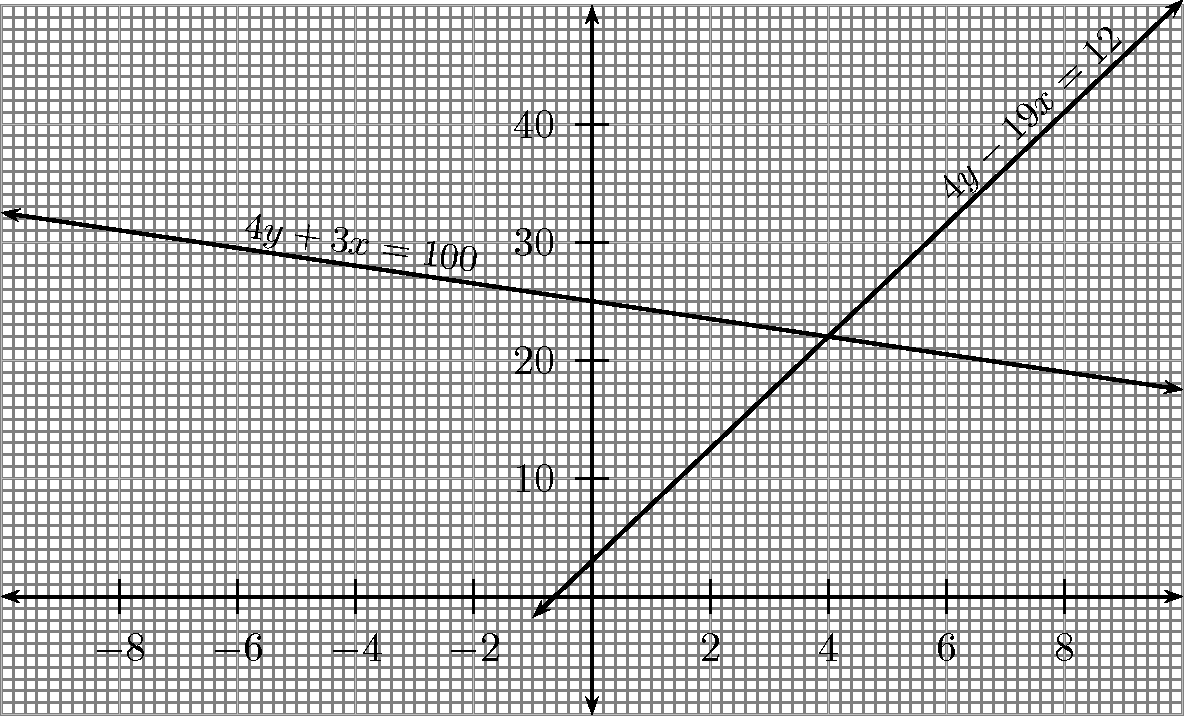
\includegraphics{col11306.imgs/m39257_MG10C10_007.png} % ;MG10C10\_007.png;;;6.0;8.5;
\begin{center}
\begin{pspicture}(-5,-1)(5,5)
%  \psgrid[subgriddiv=10,gridcolor=lightgray,gridlabels=0,gridwidth=0.1pt]
\psaxes[dx=1,dy=1,Dy=10,Dx=2,arrows=<->](0,0)(-5,-1)(5,5)
\pstextpath[c](-2,0.1){\psplot[xunit=0.5,yunit=0.1,plotstyle=curve,arrows=<->]{-10}{10}{0.75 x mul neg 25 add}}{\small{$4y+3x=100$}}
\pstextpath[c](2.2,0.1){\psplot[xunit=0.5,yunit=0.1,plotstyle=curve,arrows=<->]{-1}{10}{4.75 x mul 3 add}}{\small{$4y-19x=12$}}
\end{pspicture}
\end{center}

\vspace{2pt}
\vspace{.1in}
\end{center}
\end{figure}         

\westep{Find the coordinates of the point of intersection}
The two graphs intersect at $(4;22)$ 

\westep{Write the final answer}
\begin{equation*}
\begin{array}{ccl}\hfill x& =& 4\hfill \\ \hfill y& =& 22\hfill \end{array}
\end{equation*}

}
\end{wex}

\begin{exercises}{}
{
 \Note{Solving a system of simultaneous equations graphically is sometimes not very accurate but provides a valuable method of solution.}
\item Solve algebraically: 
\begin{enumerate}[noitemsep, label=\textbf{\arabic*}. ] 
\item $3x-14y=0$ , $x-4y+1=0$
\item $x+y=8$, $3x + 2y = 21$
\item $y=2x+1$ , $x + 2y + 3 = 0$
\end{enumerate}

Solve graphically and check your answer algebraically:

\begin{enumerate}[noitemsep, label=\textbf{\arabic*}. ] 
\setcounter{enumi}{3}
\item  $x+2y=1$, $\frac{x}{3} + \frac{y}{2} = 1$
\item $5= x+y$ , $-x = y-2$
\item $3x - 2y = 0$ , $x - 4y + 1 = 0$

\end{enumerate}


\par \raisebox{-5 pt}{
\includegraphics[width=0.5cm]{col11306.imgs/summary_www.png}} Find the answers with the shortcodes:
\par \begin{tabular}[h]{cccccc}
(1.) lxq  &  (2.) lxl  &  (3.) lxi  &  (4.) lx3  & \end{tabular}
}
\end{exercises}

\section{Word problems}

$ \hspace{-5pt}\begin{array}{cccccccccccc}   
\includegraphics[width=0.75cm]{col11306.imgs/summary_fullmarks.png} &   \end{array} $ \hspace{2 pt}\raisebox{-5 pt}{} {(section shortcode: MG10079 )} \par

To solve word problems we need to write a set of equations that represent the problem mathematically. 
The solution of the equations is then the solution to the problem.

\subsection*{Problem solving strategy}

\begin{enumerate}[noitemsep, label=\textbf{\arabic*}. ] 
\item Read the whole the question.
\item What are we asked to solve for?
\item Assign a variable to the unknown quantity e.g., $x$.
\item  Translate the words into algebraic expressions by rewriting the given information in terms of the variable. 
\item Set up an equation or system of equations to solve for the variable.
\item Solve the equation algebraically using substitution.
\item Check the solution.
\end{enumerate}

\begin{wex}
{Solving word problems}
{
A shop sells bicycles and tricycles. In total there are $7$ cycles (cycles include both bicycles and tricycles) and $19$ wheels. Determine how many of each there are, if a bicycle has two wheels and a tricycle has three wheels.
}
{
\westep{Assign variable to unknown}
Let $b$ be the number of bicycles \\
and let $7-b$ be the number of tricycles. 

\westep{Set up an equation}
\begin{equation*}
\begin{array}{ccc}\hfill 2b+3(7-b)& =& 19\hfill \end{array}
\end{equation*}


\westep{Rearrange and solve for $b$}
\begin{equation*}
\begin{array}{ccl}
 \hfill 2b + 21 - 3b& =& 19\hfill \\
\hfill - b& =& -2\hfill \\
 \hfill \therefore b& =& 2\hfill 
\end{array}
\end{equation*}

\westep{Calculate number of tricycles}
\begin{equation*}
\begin{array}{ccl}
\\ \hfill  7 - 2 & =& 5\hfill \\
 \therefore \mbox{ Number of tricycles }& =& 5
\end{array}
\end{equation*}

\westep{Write final answer}
 There are $5$ tricycles and $2$ bicycles.

}       
\end{wex}

\begin{wex}{Solving word problems}{
Bongani and Jane are friends. Bongani takes Jane's physics test paper and will not tell her what her mark is. 
He knows that Jane hates maths so he decides to tease her. Bongani says: 'I have $2$ marks more than you do and the sum of both our marks is equal to $14$. 
How much did we get?'}
{
\westep{Assign variables to the unknowns}
We have two unknowns, Bongani's mark and
 Jane's mark. 
\\Let Bongani's mark be $t$ and Jane's mark be $j$. 

\westep{Set up a system of equations}
\\Bongani has $2$ more marks than Jane.
\begin{equation*}
t=j+2
\end{equation*}

Both marks add up to $14$.

\begin{equation*}
t+j=14
\end{equation*}

\westep{Use the first equation to express $t$ in terms of $j$}
\begin{equation*}
t=j+2
\end{equation*}

\westep{Substitute into second equation}
\begin{equation*}
    \begin{array}{ccc}\hfill t+j& =& 14\hfill \\
	\hfill (j+2)+j& =& 14\hfill \\

    \end{array}
\end{equation*}

\westep{Rearrange and solve for $j$}
\begin{equation*}
    \begin{array}{ccl}\hfill 2j& =& 14 - 2\hfill \\
	\hfill \therefore 2j& =& 12\hfill \\
\hfill \therefore j &=& 6 \hfill

    \end{array}
\end{equation*}

 \westep{Substitute value for $j$ back into first equation and solve for $t$}
\begin{equation*}
\begin{array}{ccl}\hfill t& =& j+2\hfill \\ & =& 6+2\hfill \\ & =& 8\hfill \end{array}
\end{equation*}
\\
\westep{Check the solution satisfies both original equations}
\westep{Write the final answer}
Bongani got $8$ for his test and Jane got  $6$.\\
}
\end{wex}

\begin{wex}
{Solving word problems}
{
A fruit shake costs R$~2,00$ more than a chocolate milkshake. If three fruit shakes and $5$ chocolate milkshakes cost R$~78,00$, determine the individual prices.}

{
\westep{Assign variables to unknowns}  
Let the price of a chocolate milkshake be $x$ 
\\ and let the price of a fruitshake be $y$.


\westep{Set up a system of equations}
\begin{equation*}
\begin{array}{ccl} \hfill y &=& x+2 \hfill \\
\hfill 3y+5x& =& 78\hfill 
\end{array}
\end{equation*}

\westep{Substitute first equation into the second}
\begin{equation*}
\begin{array}{ccl}\hfill 3(x+2)+5x& =& 78\hfill \\
\end{array}
\end{equation*}

\westep{Rearrange and solve for $x$}
\begin{equation*}
\begin{array}{ccl}
 \hfill 3x+6+5x& =& 78\hfill \\ 
\hfill 8x& =& 72\hfill \\ 
\hfill \therefore x& =& 9\hfill \\  \end{array}
\end{equation*}

\westep{Substitute value for $x$ back into first equation and solve for $y$}
\begin{equation*}
\begin{array}{ccl}
\hfill y& =& x+2\hfill \\
 \hfill & =& 9+2\hfill \\ 
\hfill & \therefore =& 11\hfill  \end{array}
\end{equation*}
\westep{Check the solution satisfies both original equations}
\westep{Write final answer}
One chocolate milkshake costs R$~9,00$ and one fruitshake costs R$~ 11,00$.
}
\end{wex}

\begin{wex}
{Solving word problems }
{
The product of two consecutive negative integers is $1122$. Find the two integers.
} 
{
\westep{Assign variable to unknown}
Let the first integer be $n$ 
\\and let the second integer be $n+1$.\par 

\westep{Set up an equation}  
\begin{equation*}
\begin{array}{cll}\hfill n(n+1)& =& 1122\hfill \end{array}
\end{equation*}

\westep{Expand and solve for $n$}
\begin{equation*}
    \begin{array}{cll}
	\hfill n^{2} + n =& 1122\hfill \\
\hfill n^{2} + n - 1122 =& 0\hfill \\
\hfill (n+34)(n-33) =& 0\hfill \\
	\hfill \therefore  n =& -34 \hfill \\
\hfill \mbox{ or } n =& 33\hfill 
    \end{array}
\end{equation*}

\westep{Integers must be negative}
\begin{equation*}
    \begin{array}{cll}
	\hfill \therefore n =& -34\hfill \\
\hfill n + 1 =& -34\ + 1 \hfill \\
\hfill  =& -33\hfill \\

    \end{array}
\end{equation*}

\westep{Write final answer} 
The two consecutive negative numbers are $-34$ and $-33$.
}
\end{wex}

\begin{exercises}{Word problems}
{
\begin{enumerate}[noitemsep, label=\textbf{\arabic*}. ] 
\item Two jets are flying towards each other from airports that are $1~200$ km apart. One jet is flying at $250$ km/h and the other jet at $350$ km/h. If they took off at the same time, how long will it take for the jets to pass each other?
\item Kadesh bought $20$ shirts at a total cost of R$~980$. If the large shirts cost R$~50$ and the small shirts cost R$~40$, how many of each size did he buy?
\item The diagonal of a rectangle is $25~$cm more than its width. The length of the rectangle is $17~$cm more than its width. What are the dimensions of the rectangle?  
\item The sum of $27$ and $12$ is equal to $73$ more than an unknown number. Find the unknown number.
\item The two smaller angles in a right-angled triangle are in the ratio of $1:2$. What are the sizes of the two angles? 
\item The length of a rectangle is twice the breadth. If the area is $128$ cm$^{2}$, determine the length and the breadth.       
\item If $4$ times a number is increased by $7$, the result is $15$ less than the square of the number. Find the number.
\item The length of a rectangle is $2~$cm more than the width of the rectangle. The perimeter of the rectangle is $20~$cm. Find the length and the width of the rectangle.
\item Stephen has $1~l$ of a mixture containing $69\%$ of salt. How much water must Stephen add to make the mixture $50\%$ salt? Write your answer as a fraction of a litre.
       
\end{enumerate}

\par \raisebox{-5 pt}{
\includegraphics[width=0.5cm]{col11306.imgs/summary_www.png}} Find the answers with the shortcodes:
\par \begin{tabular}[h]{cccccc}
(1.) lcy  &  (2.) lcV  &  (3.) lcp  &  (4.) lcw  &  (5.) lcd  &  (6.) lcf  &  (7.) lcv  & \end{tabular}
}
\end{exercises}

\section{Literal equations}
 $ \hspace{-5pt}\begin{array}{cccccccccccc}   
\includegraphics[width=0.75cm]{col11306.imgs/summary_fullmarks.png} &   \end{array} $ \hspace{2 pt}\raisebox{-5 pt}{} {(section shortcode: MG10078 )}\par
%   \label{m39258*eip-798}
%             \ssection{ Equations and inequalities: Literal equations}
%             \nopagebreak
%             

A literal equation is one that has several letters or variables. Examples include the area of a circle ($A=\pi{r}^{2}$) and the formula for speed ($s=\frac{d}{t}$). In this section we solve literal equations in terms of one variable. To do this, we use the principles we have learnt about solving equations and apply them to rearranging literal equations. Solving literal equations is also known as changing the subject of the formula.
 
Keep the following in mind when solving literal equations:
\begin{itemize}
\item We isolate the unknown variable by asking 'what is it joined to?' and 'how is it joined?' We then perform the opposite operation to both sides as a whole.
\item If the unknown variable is in two or more terms, then we take it out as a common factor. 
\item  If we have to take the square root of both sides, remember that there will be a positive and a negative answer.
\item  If the unknown variable is in the denominator, we multiply both sides by the lowest common denominator (LCD) and then continue to solve.
\end{itemize}


\begin{wex}
{Solving literal equations}
{
The area of a triangle is $A=\frac{1}{2}bh$. What is the height of the triangle in terms of the base and area?
}
{
\westep{Isolate the required variable}
We are asked to isolate the height so  rearrange the equation with $h$ on one side of the equals sign and the rest of the variables on the other.
\begin{equation*}
    \begin{array}{cccc}\hfill A& =& \frac{1}{2}bh\hfill & \\
	\hfill 2A& =& bh\hfill & \hfill \\
	\hfill \frac{2A}{b}& =& h\hfill 
    \end{array}
\end{equation*}

\westep{Write the final answer} 
The height of a triangle is given by: $h=\dfrac{2A}{b}$
} 
\end{wex}

\begin{wex}
{Solving literal equations}
{
Given the formula $h=\dfrac{H}{R+r} \times R$, solve for $R$.
}
{
\westep{Isolate the required variable}
\begin{equation*}
    \begin{array}{ccll}\hfill h(R+r)& =& H \times R\hfill & \\
	\hfill hR + hr& =& HR\hfill & \hfill \\
	\hfill hr & =& HR - hR\hfill \\
\hfill hr& =& R(H - h)\hfill \vspace{5pt}\\ 
\hfill \therfore R & =& \dfrac{hr}{H-h}\hfill 
    \end{array}
\end{equation*}

\westep{Write the final answer} 
$R = \dfrac{hr}{H-h}$
} 
\end{wex}


\begin{exercises}{}
{
\begin{enumerate}[noitemsep, label=\textbf{\arabic*}. ] 
\item Solve for $t$: $v=u+at$
\item Solve for $x$: $ax-bx=c$ \vspace{5pt}
\item Solve for $x$: $\dfrac{1}{b}+\dfrac{2b}{x}=2$\vspace{5pt}
\item Solve for $r$: $V = \pi r^{2} h$
\item Write $l$ in terms of $b$ and $H$: $\sqrt{l^{2}+b^{2}}=H$
\item Solve for $i$: $A=P(1+i)^{n}$
\item Solve for $h$: $A=2\pi rh + 2 \pi r$
\item Solve for $b$: $V=l \times b \times h$
\item Solve for $h$: $V=\frac{1}{3}\pi r^{2}h$
\end{enumerate}

\par \raisebox{-5 pt}{
\includegraphics[width=0.5cm]{col11306.imgs/summary_www.png}} Find the answers with the shortcodes:
\par \begin{tabular}[h]{cccccc}
(1.) lgw  &  (2.) lgw  &  (3.) lgw  & \end{tabular}
}
\end{exercises}

\section{Solving linear inequalities}
\nopagebreak
$ \hspace{-5pt}\begin{array}{cccccccccccc}   
\includegraphics[width=0.75cm]{col11306.imgs/summary_fullmarks.png} &   
\includegraphics[width=0.75cm]{col11306.imgs/summary_video.png} &   \end{array} $ \hspace{2 pt}\raisebox{-5 pt}{} {(section shortcode: MG10073 )} \par 


\begin{activity}{Linear inequalities}
{
Represent the following on number lines and using interval notation:
\begin{enumerate}[noitemsep, label=\textbf{\arabic*}. ] 
\item $x<4$
\item $x\leq 4$
\item $x\geq 4$
\item $x>4$
\end{enumerate}
}
\end{activity}

A linear inequality is similar to a linear equation in that the largest exponent of a variable is $1$. The following are examples of linear inequalities.\par 

\begin{equation*}
\begin{array}{ccc}\hfill 2x+2& \leq& 1\hfill \\ \hfill \dfrac{2-x}{3x+1}&\geq& 2\hfill \\ \hfill \frac{4}{3}x-6&<& 7x+2\hfill \end{array}
\end{equation*}
The methods used to solve linear inequalities are similar to those used to
solve linear equations. The only difference occurs when there is a
multiplication or a division that involves a minus sign. For example, we know
that $8>6$. If both sides of the inequality are divided by $-2$ the we get $-4 > -3$ which is not true. Therefore, the inequality sign must be switch around, giving
$-4<-3$.

\Tip{When we divide or multiply both sides of an inequality by any number with
a minus sign, the direction of the inequality changes. For this reason we cannot divide or multiply by a variable.}

For example, if $x<1$, then $-x>-1$.
In order to compare an inequality to a normal equation, we shall solve an equation first. Solve $2x+2=1$.

\begin{equation*}
\begin{array}{ccl}\hfill 2x+2& =& 1\hfill \\ \hfill 2x& =& 1-2\hfill \\ \hfill 2x& =& -1\hfill \\ \hfill x& =& -\frac{1}{2}\hfill \end{array}
\end{equation*}
If we represent this answer on a number line, we get\par 

\setcounter{subfigure}{0}
\begin{figure}[H] % horizontal\label{m39254*id157630}
\begin{center}
\label{m39254*id157630!!!underscore!!!media}\label{m39254*id157630!!!underscore!!!printimage}
%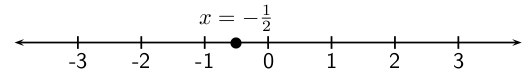
\includegraphics[width=.8\columnwidth]{col11306.imgs/m39254_MG10C10_001.png} % m39254;MG10C10\_001.png;;;6.0;8.5;
\begin{center}
\begin{pspicture}(-4,0.75)(4,1.75)
%\psgrid
\psline[arrows=<->](-4,1)(4,1)
\psdot[dotsize=5pt](-0.5,1)
\multido{\n=-3+1}{7}
{\uput[d](\n,1){$\n$}
\psline(\n,1.1)(\n,0.9)}
\uput[u](-0.5,1){$x=-\frac{1}{2}$}
\end{pspicture}
\end{center}
\vspace{2pt}
\vspace{.1in}
\end{center}
\end{figure}       
\par 
Now let us solve the inequality $2x+2\leq1$.\par 


\begin{equation*}
\begin{array}{ccl}\hfill 2x+2& \leq& 1\hfill \\ \hfill 2x& \leq& 1-2\hfill \\ \hfill 2x& \leq& -1\hfill \\ \hfill x& \leq& -\frac{1}{2}\hfill \end{array}
\end{equation*}
If we represent this answer on a number line, we get\par 

\setcounter{subfigure}{0}
\begin{figure}[H] % horizontal\label{m39254*id157774}
\begin{center}
\label{m39254*id157774!!!underscore!!!media}\label{m39254*id157774!!!underscore!!!printimage}
%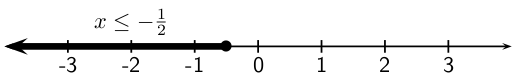
\includegraphics[width=.8\columnwidth]{col11306.imgs/m39254_MG10C10_002.png} % m39254;MG10C10\_002.png;;;6.0;8.5;
\begin{center}
\begin{pspicture}(-4,0.75)(4,1.75)
%\psgrid
\psline[arrows=<->](-4,1)(4,1)
\psdot[dotsize=5pt](-0.5,1)
\multido{\n=-3+1}{7}
{\uput[d](\n,1){$\n$}
\psline(\n,1.1)(\n,0.9)}
\uput[u](-2,1){$x\le-\frac{1}{2}$}
\psline[linewidth=3pt]{->}(-0.5,1)(-4,1)
\end{pspicture}
\end{center}
\vspace{2pt}
\vspace{.1in}
\end{center}
\end{figure}       
\par 

If we represent this answer in interval notation we write $(-\infty ~;-\frac{1}{2}]$.\par
\Note{Assume $x \in \mathbb{R}$ if the set of numbers to be used is not specified.}
We see that for the equation there is only a single value of $x$ for which the equation is true. However, for the inequality, there is a range of values for which the inequality is true. This is the main difference between an equation and an inequality.\par 

\setcounter{subfigure}{0}
\begin{figure}[H] % horizontal\label{m39254*inequalities-1}
\textnormal{Khan academy video on inequalities - 1}\vspace{.1in} \nopagebreak
\label{m39254*yt-media4}\label{m39254*yt-video4}
\raisebox{-5 pt}{ 
\includegraphics[width=0.5cm]{col11306.imgs/summary_www.png}} { (Video:  MG10074 )}
\vspace{2pt}
\vspace{.1in}
\end{figure}    

\setcounter{subfigure}{0}
\begin{figure}[H] % horizontal\label{m39254*inequalities-2}
\textnormal{Khan academy video on inequalities - 2}\vspace{.1in} \nopagebreak
\label{m39254*yt-media5}\label{m39254*yt-video5}
\raisebox{-5 pt}{ 
\includegraphics[width=0.5cm]{col11306.imgs/summary_www.png}} { (Video:  MG10075 )}
\vspace{2pt}
\vspace{.1in}
\end{figure}  
  
\begin{wex}
{Sovling linear inequalities }
{
Solve for $r$: $6-r>2$ \\
Represent answer on a number line and in interval notation.}
{ 
\westep{Rearrange and solve for $r$}  
\begin{equation*}
\begin{array}{ccl}\hfill -r&>&2-6\\ \hfill -r&>&-4\end{array}
\end{equation*}
\westep{Multiply by a minus sign and switch around the inequality sign}

\begin{equation*}
r<4
\end{equation*}
(Remember: when you multiply by a minus sign, the direction of the inequality changes.)

\westep{Represent answer on a number line}

\setcounter{subfigure}{0}
\begin{figure}[H] % horizontal\label{m39254*id157937}
\begin{center}

%\includegraphics{col11306.imgs/m39254_MG10C10
% _003.png} % ;MG10C10\_003.png;;;6.0;8.5;
\begin{center}
\begin{pspicture}(-1,0.4)(6,1.6)
%\psgrid
\psline[arrows=<->](-1,1)(6,1)
\multido{\n=0+1}{6}
{\uput[d](\n,1){$\n$}
\psline(\n,1.1)(\n,0.9)}
\uput[u](2,1){$r<4$}
\psline[linewidth=3pt]{->}(4,1)(-1,1)
\psdot[dotsize=5pt,dotstyle=o](4,1)
\end{pspicture}
\end{center}
}
\vspace{2pt}
\vspace{.1in}
\end{center}
\end{figure}    

\westep{Represent answer in interval notation}
\begin{equation*}
(- \infty~;~4)   
\end{equation*}
}
\end{wex}

\begin{wex}{Solving linear inequalities }
{
Solve for $q$: $4q+3<2(q+3)$ \\
Represent answer on a number line and in interval notation.
}
{
\westep{Expand the bracket}  
\begin{equation*}
\begin{array}{ccl}\hfill 4q+3& <& 2(q+3)\hfill \\ \hfill 4q+3& <& 2q+6\hfill \end{array}
\end{equation*}

\westep{Rearrange and solve for $q$}
\begin{equation*}
\begin{array}{ccl}\hfill 4q+3& <& 2q+6\hfill \\ \hfill 4q-2q& <& 6-3\hfill \\ \hfill 2q& <& 3\hfill \end{array}
\end{equation*}


\westep{Divide both sides by $2$}  
\begin{equation*}
\begin{array}{ccccc}\hfill 2q& <& 3\hfill &  \\ \hfill q& <& \frac{3}{2}\hfill & \end{array}
\end{equation*}

\westep{Represent answer on a number line} 

\setcounter{subfigure}{0}
\begin{figure}[H] % horizontal\label{m39254*id158287}
\begin{center}
\label{m39254*id158287!!!underscore!!!media}\label{m39254*id158287!!!underscore!!!printimage}
%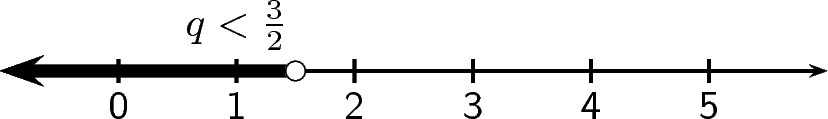
\includegraphics{col11306.imgs/m39254_MG10C10_004.png} % ;MG10C10\_004.png;;;6.0;8.5;
\begin{center}
\begin{pspicture}(-1,0.4)(6,1.6)
%\psgrid
\psline[arrows=<->](-1,1)(6,1)
\multido{\n=0+1}{6}
{\uput[d](\n,1){$\n$}
\psline(\n,1.1)(\n,0.9)}
\uput[u](1,1){$q<\frac{3}{2}$}
\psline[linewidth=3pt]{->}(1.5,1)(-1,1)
\psdot[dotsize=5pt,dotstyle=o](1.5,1)
\end{pspicture}
\end{center}

\vspace{2pt}
\vspace{.1in}
\end{center}
\end{figure}   

\westep{Represent answer in interval notation}
\begin{equation*}
(- \infty~;~\frac{3}{2})
\end{equation*}
}
\end{wex}


\begin{wex}
{Solving compound linear inequalities }
{Solve for $x$: $5\leq x+3<8$ \\
Represent answer on a number line and in interval notation.}  
{
\westep{Subtract $3$ from all terms}
\begin{equation*}
\begin{array}{cccll}\hfill 5-3 &\leq& x+3-3 &<& 8-3\hfill \\
		  \hfill 2&\leq& x &<&5 \hfill
\end{array}
\end{equation*}

\westep{Represent answer on a number line}

\setcounter{subfigure}{0}
\begin{figure}[H] % horizontal\label{m39254*id158459}
\begin{center}
\label{m39254*id158459!!!underscore!!!media}\label{m39254*id158459!!!underscore!!!printimage}
%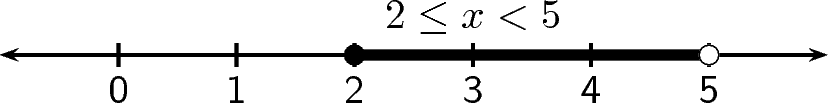
\includegraphics{col11306.imgs/m39254_MG10C10_005.png} % ;MG10C10\_005.png;;;6.0;8.5;
\begin{center}
\begin{pspicture}(-1,0.4)(6,1.6)
%\psgrid
\psline[arrows=<->](-1,1)(6,1)
\multido{\n=0+1}{6}
{\uput[d](\n,1){$\n$}
\psline(\n,1.1)(\n,0.9)}
\uput[u](3,1){$2\le x < 5$}
\psline[linewidth=2.5pt](2,1)(5,1)
\psdot[dotsize=5pt,dotstyle=o](5,1)
\psdot[dotsize=5pt](2,1)
\end{pspicture}
\end{center}

\vspace{2pt}
\vspace{.1in}
\end{center}
\end{figure}       
}

\westep{Represent answer in interval notation}
\begin{equation*}
[~2~;~5)
\end{equation*}
\end{wex}


\begin{exercises}{ }
{
Solve for $x$ and represent the answer on a number line and in interval notation:
\begin{enumerate}[noitemsep, label=\textbf{\arabic*}. ] 

    \item $3x+4>5x+8$
    \item $3(x-1)-2\leq 6x+4$ \vspace{5pt}
    \item $\dfrac{x-7}{3}>\dfrac{2x-3}{2}$\vspace{5pt}
    \item $-4(x-1)<x+2$\vspace{5pt}
    \item $\dfrac{1}{2}x+\dfrac{1}{3}(x-1)\geq \dfrac{5}{6}x-\dfrac{1}{3}$ \vspace{5pt}
    \item $-2\leq x-1<3$ 
    \item $-5<2x-3\leq7$ 
\item $7(3x+2)-5(2x-3)>7$
    \end{enumerate}


\par \raisebox{-5 pt}{
\includegraphics[width=0.5cm]{col11306.imgs/summary_www.png}} Find the answers with the shortcodes:
\par \begin{tabular}[h]{cccccc}
(1.) lcJ  &  (2.) lcS  &  (3.) lch  & \end{tabular}
}
\end{exercises}

\summary
\nopagebreak
\label{m39263} $ \hspace{-5pt}\begin{array}{cccccccccccc}   \end{array} $ \hspace{2 pt}\raisebox{-5 pt}{
\includegraphics[width=0.5cm]{col11306.imgs/summary_www.png}} {(section shortcode: MG10080 )} \par 

\begin{itemize}[noitemsep]
\item A linear equation is an equation where the exponent of the variable is $1$. A linear equation has at most one solution.
\item A quadratic equation is an equation where the exponent of the variable is at most $2$. A quadratic equation has at most two solutions.
\item A linear inequality is similar to a linear equation and has the exponent of the variable equal to $1$.
\item If we divide or multiply both sides of an inequality by any number with a minus sign, the direction of the inequality changes. 
\item To solve for two unknown variables, two equations are required.These equations are known as a system simultaneous equations. There are two ways to solve linear simultaneous equations: algebraic solutions and graphical solutions.To solve algebraically we use substitution or elimination methods. To solve graphically we draw the graph of each equation and the solution will be the co-ordinates of the point of intersection. 
\item Literal equations are equations that have several letters and variables.
\item Word problems require a set of equations that represent the problem mathematically. 
\end{itemize}

\begin{eocexercises}{}
{
 Solve:
\begin{enumerate}[noitemsep, label=\textbf{\arabic*}. ] 
\begin{multicols}{2} 
\item $2(p-1) = 3(p+2)$
\item $3-6k = 2k-1$
\item $m + 6(-m+1) + 5m = 0$
\item $2k + 3 = 2-3(k+3)$
\item $5t-1=t^{2}-(t+2)(t-2)$\vspace{5pt}
\item $3+\dfrac{q}{5} = \dfrac{q}{2}$ \vspace{5pt}
\item $5-\dfrac{2(m+4)}{m} = \dfrac{7}{m}$\vspace{5pt}
\item $\dfrac{2}{t} - 2 - \dfrac{1}{2} = \dfrac{1}{2}(1+\dfrac{2}{t})$\vspace{5pt}
\item $x^{2} - 3x + 2=0$
\item $y^{2} + y = 6$
\item $0=2x^{2} - 5x - 18$\vspace{5pt}
\item $(d+4)(d-3)-d=(3d-2)^{2} - 8d(d-1)$\vspace{5pt}
\item $5x+2\leq4(2x-1)$\vspace{5pt}
\item $\dfrac{4x-2}{6} > 2x+1$\vspace{5pt}
\item $\dfrac{x}{3} - 14 > 14 - \dfrac{x}{7}$\vspace{5pt}
\item $\dfrac{1-a}{2} - \dfrac{2-a}{3} \geq 1$\vspace{5pt}
\item $-5 \leq 2k + 1 < 5$\vspace{5pt}
\item $x-1=\dfrac{42}{x}$  
\end{multicols}
\end{enumerate}

Consider the following literal equations:
\begin{enumerate}[noitemsep, label=\textbf{\arabic*}. ] 
\setcounter{enumi}{18}
\item Solve for $i$: $P = VI$
\item Solve for $m$: $E=mc^{2}$
\item Solve for $t$: $v = u + at$\vspace{5pt}
\item Solve for $f$: $\dfrac{1}{u} + \dfrac{1}{v} = \dfrac{1}{f}$\vspace{5pt}
\item Solve for $C$: $F=\frac{9}{5}C + 32$\vspace{5pt}
\item Solve for $y$: $m = \dfrac{y-c}{x}$\vspace{5pt}
\end{enumerate}

Solve the following simultaneous equations:
\begin{enumerate}[noitemsep, label=\textbf{\arabic*}. ] 
\setcounter{enumi}{24}
\item $7x+3y=13$ and $2x-3y=-4$  
\item $10=2x+y$ and $y=x-2$
\item $7x-41=3y$ and $17=3x-y$
\item $2y=x+8$ and $4y=2x-44$
\end{enumerate}

Find the solutions to the following word problems:
\begin{enumerate}[noitemsep, label=\textbf{\arabic*}. ] 
\setcounter{enumi}{28}
\item $\frac{7}{8}$ of a certain number is $5$ more than of $\frac{1}{3}$ of the number. Find the number.
\item Three rulers and two pens have a total cost of R $21,00$. One ruler and one pen have a total cost of R $8,00$. How much does a ruler cost and how much does a pen cost? 
\item A man runs to the bus stop and back in $15$ minutes. His speed on the way to the bus stop is $5$ km/h and his speed on the way back is $4$ km/h. Find the distance to the bus stop.
\item Zanele and Piet skate towards each other on a straight path. They set off $20$ km apart. Zanele skates at $15$ km/h and Piet at $10$ km/h. How far will Piet have skated when they reach each other?
\item When the price of chocolates is increased by R $10$, we can buy five fewer chocolates for R $300$. What was the price of each chocolate before the price was increased?
   
\end{enumerate}
\end{enumerate}

\par \raisebox{-5 pt}{
\includegraphics[width=0.5cm]{col11306.imgs/summary_www.png}} Find the answers with the shortcodes:
\par \begin{tabular}[h]{cccccc}
(1.) lcG  &  (2.) lc7  &  (3.) lcA  &  (4.) lco  &  (5.) lcs  &  (6.) lcH  &  (7.) lc6  &  (8.) lcF  &  (9.) lcL  &  (10.) lcM  & \end{tabular}
}
\end{eocexercises}